\documentclass{article}
\usepackage{indentfirst}
\usepackage[utf8]{inputenc}
\usepackage[T1]{fontenc}
\usepackage[brazilian]{babel}
\usepackage{lmodern}
\usepackage{graphicx}
\usepackage{float}
\usepackage[]{subfigure}
\usepackage{afterpage}
\usepackage{amsmath}
\usepackage{mathrsfs}
\usepackage{textcomp,gensymb}
\usepackage{nameref}
\usepackage{accents}
\usepackage{listings}
\usepackage{color,soul}
\usepackage[margin=1in]{geometry}
\usepackage{steinmetz}
\usepackage{xfrac}

%\PassOptionsToPackage{hyphens}{url}\usepackage{hyperref}
%\hypersetup{
    %breaklinks = true,
%}
%\urlstyle{same}
\newcommand{\ubar}[1]{\underaccent{\bar}{#1}}
%\renewcommand\thesection{\arabic{section}$^a$}
\renewcommand\thesection{\arabic{section}.}
\renewcommand\thesubsection{\arabic{section}.\alph{subsection}}
\definecolor{dkgreen}{rgb}{0,0.6,0}
\definecolor{gray}{rgb}{0.5,0.5,0.5}
\definecolor{mauve}{rgb}{0.58,0,0.82}
\lstset{
    frame=tb,
    language=Matlab,
    aboveskip=3mm,
    belowskip=3mm,
    showstringspaces=false,
    basicstyle={\small\ttfamily},
    numbers=none,
    numberstyle=\tiny\color{gray},
    keywordstyle=\color{blue},
    commentstyle=\color{dkgreen},
    stringstyle=\color{mauve},
    breaklines=true,
    breakatwhitespace=true,
    tabsize=4
}

\DeclareMathOperator\det{det}
\DeclareMathOperator\adj{adj}

\title{Simulação 6 - Controle Digital}
\author{Arthur de Matos Beggs - 12/0111098}
\date{2021}

\begin{document}
% capa
\begin{titlepage}
    \begin{center}
        \centering
        
\includegraphics[width=.7\linewidth]{images/logo_unb.png}\\[0.5cm]
        {\large \textbf{Universidade de Brasília}}\\[0.2cm]
        {\large \textbf{Departamento de Engenharia Elétrica}}\\[0.2cm]
        {\large \textbf{Controle Digital}}\\[4.8cm]
        {\bf \huge {Exercício de Simulação 6}}\\[0.2cm]
        {\bf \large {}}
    \end{center}

    \vspace{5cm}
    \hspace{2cm} {\noindent \bf \large {Aluno:}}\\
    \vspace{0.8cm}
    \hspace{2.35cm} {\large Arthur de Matos Beggs --------------------------------- 12/0111098}\\[1cm]

    \begin{center}
        {\large Brasília}\\
        {\large 2$^{\ubar{\circ}}$/2020}
    \end{center}

\end{titlepage}

\clearpage % Quebra de página

\setcounter{page}{2}

{Um sistema a tempo discreto é descrito por}
\begin{align*}
    x[k+1] &= Gx[k] + H_1u[k] + H_2v[k],\\
    y[k] &= Cx[k],
\end{align*}
{onde}
\[
    x[k] =
    \begin{bmatrix}
        x_1[k]\\
        x_2[k]
    \end{bmatrix}
    ,\quad
    G =
    \begin{bmatrix}
        0.5 && 1\\
        0.5 && 0.7
    \end{bmatrix}
    ,\quad
    H_1 =
    \begin{bmatrix}
        0.2\\
        0.1
    \end{bmatrix}
    ,\quad
    H_2 =
    \begin{bmatrix}
        1\\
        0
    \end{bmatrix}
    ,\quad
    C =
    \begin{bmatrix}
        1 && 0
    \end{bmatrix}
    ,\quad
\]
{$u[k]$ é a entrada e $v[k]$ é uma perturbação.}\\

{Para $y[k]$ e $x[k]$ medidos:}
\section{\normalsize \normalfont{Determine uma realimentação de estados
$u[k] = Nr[k] - Fx[k]$ de modo que os polos de malha fechada fiquem em
$z = 0.5 \pm j0.5$ e o erro estacionário seja nulo quando $r[k]$ for um degrau
e $v[k] = 0$. Simule o sistema para $r[k]$ degrau unitário e $v[k] = 0$, e para
$r[k] = 0$ e $v[k]$ degrau unitário. Para cada simulação, apresente os gráficos
de $x_1[k]$, $x_2[k]$, $u[k]$ e $e[k] = r[k] - y[k]$:}}

    \begin{figure}[H]
        \centering
        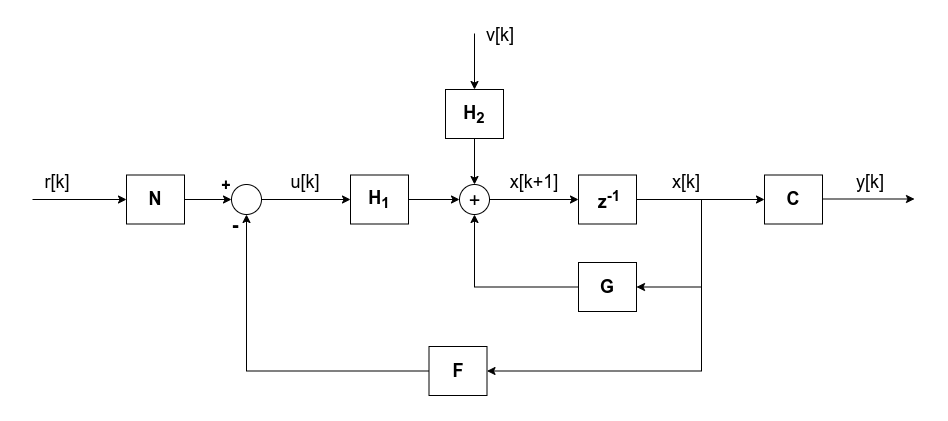
\includegraphics[width=1\linewidth]{images/diagram_q1.png}
        \caption{Diagrama do sistema.}\label{fig:diagram_q1}
    \end{figure}

    {Para que o sistema seja controlável, $\det \mathscr{C} \ne 0$}
    \[ \mathscr{C} =
        \begin{bmatrix}
            H_1 && GH_1
        \end{bmatrix} =
        \begin{bmatrix}
            0.2 && 0.2\\
            0.1 && 0.17
        \end{bmatrix};\quad
        \det \mathscr{C} = 0.014
    \]
    {Assim, o par $(G, H_1)$ é controlável.}

    {Os polos de malha fechada desejados são $\Delta_f(z) =
    (z -0.5 +j0.5)(z-0.5 -j0.5) = z^2 -z +0.5 = 0$.}

    {Considerando condições iniciais nulas de $x[0]$ e perturbação $v[k] = 0$,}
    \[ x[k+1] = Gx[k] + H_1u[k];\quad u[k] = Nr[k] - Fx[k];\quad y[k] = Cx[k]\]
    \[ x[k+1] = Gx[k] + H_1( Nr[k] - Fx[k] ) = (G - H_1F)x[k] + H_1Nr[k]\]
    {Fazendo a transformada $\mathcal{Z}$,}
    \[ zX(z) + x[0] = (G-H_1F)X(z) + H_1NR(z) \implies X(z) = (zI -G +H_1F)^{-1} H_1NR(z) \]
    \[ Y(z) = CX(z) = C (zI -G +H_1F)^{-1} H_1NR(z)
        \implies \frac{Y(z)}{R(z)} = \frac{C\adj (zI -G +H_1F)H_1N}{\det(zI -G +H_1F)} \]
    {Com $F = [f_1\quad f_2]$,}
    \[ \Delta_f(z) = \det(zI -G +H_1F)
        = \det\left(
        \begin{bmatrix}
            z && 0\\
            0 && z
        \end{bmatrix}
        - \begin{bmatrix}
            0.5 && 1\\
            0.5 && 0.7
        \end{bmatrix}
        + \begin{bmatrix}
            0.2\\
            0.1
        \end{bmatrix}
        \begin{bmatrix}
            f_1 && f_2
        \end{bmatrix}
        \right)
    \]
    \[ \Delta_f(z)
        = \det\left(
        \begin{bmatrix}
            z && 0\\
            0 && z
        \end{bmatrix}
        - \begin{bmatrix}
            0.5 && 1\\
            0.5 && 0.7
        \end{bmatrix}
        + \begin{bmatrix}
            0.2f_1 && 0.2f_2\\
            0.1f_1 && 0.1f_2
        \end{bmatrix}
        \right)
    \]

    {Pelo Matlab,}
    \begin{lstlisting}
G = [[0.5 1]; [0.5 0.7]]
H1 = [0.2; 0.1]
syms z f1 f2
F = [f1 f2]
delta_f = vpa(collect(det(z*eye(2) - G + H1*F), z))
    \end{lstlisting}
    \[ \Delta_f(z) = z^2 + (0.2f_1 + 0.1f_2 - 1.2)z + (-0.04f_1 + 0.05f_2 -0.15)
        = z^2 -z +0.5
    \]
    \[  \begin{cases}
            0.2f_1 + 0.1f_2 - 1.2 = -1 \implies
                0.2f_1 +0.1f_2 = 0.2 \implies
                0.2f_1 +0.08f_1 + 1.3 = 0.2\\
            -0.04f_1 + 0.05f_2 -0.15 = 0.5 \implies
                -0.04f_1 + 0.05f_2 = 0.65 \implies
                0.1f_2 = 0.08f_1 +1.3
        \end{cases}
    \]
    \[  \begin{cases}
            f_1 = -3.9286\\
            f_2 = 9.8571
        \end{cases}
    \]
    \[ F = [-3.9286\quad 9.8571] \]

    {Para $e_{ss} = 0$ para $r[k]$ degrau unitário e $v[k] = 0$,
    $e_{ss} = e[\infty] = r[\infty] - y[\infty]$, $R(z) = \frac{1}{1-z^{-1}}$,}
    \[ y[\infty] = \lim\limits_{z \to 1} (1-z^{-1})Y(z)
        = \lim\limits_{z \to 1} (1-z^{-1})C (zI -G +H_1F)^{-1} H_1N \frac{1}{1-z^{-1}} \]
    \[ y[\infty] = C (zI -G +H_1F)^{-1} H_1N \]
    \[ e[\infty] = r[\infty] - y[\infty] = 1 - C (zI -G +H_1F)^{-1} H_1N = 0
        \implies C (zI -G +H_1F)^{-1} H_1N = 1
    \]
    \[ N = \frac{1}{C (zI -G +H_1F)^{-1} H_1} \]

    {Pelo Matlab,}
    \begin{lstlisting}
F = [ ((0.2-1.3)/0.28) ((((0.2-1.3)/0.28)*0.08 + 1.3)/0.1) ]
N = 1/(C * inv(eye(2) - G + H1*F) * H1)
    \end{lstlisting}
    \[ N = 3.125 \]
    \[ u[k] = 3.125r[k] - [-3.9286\quad 9.8571]
        \begin{bmatrix}
            x_1[k]\\
            x_2[k]
        \end{bmatrix}
    \]

    \clearpage
    {Simulando o sistema da Figura~\ref{fig:simulink_q1} no Simulink, obtemos a
    resposta da Figura~\ref{fig:q1_r1_v0} para $r[k]$ degrau unitário e $v[k]=0$,
    e a resposta da Figura~\ref{fig:q1_r0_v1} para $r[k]=0$ e $v[k]$ degrau unitário.}

    \begin{figure}[H]
        \centering
        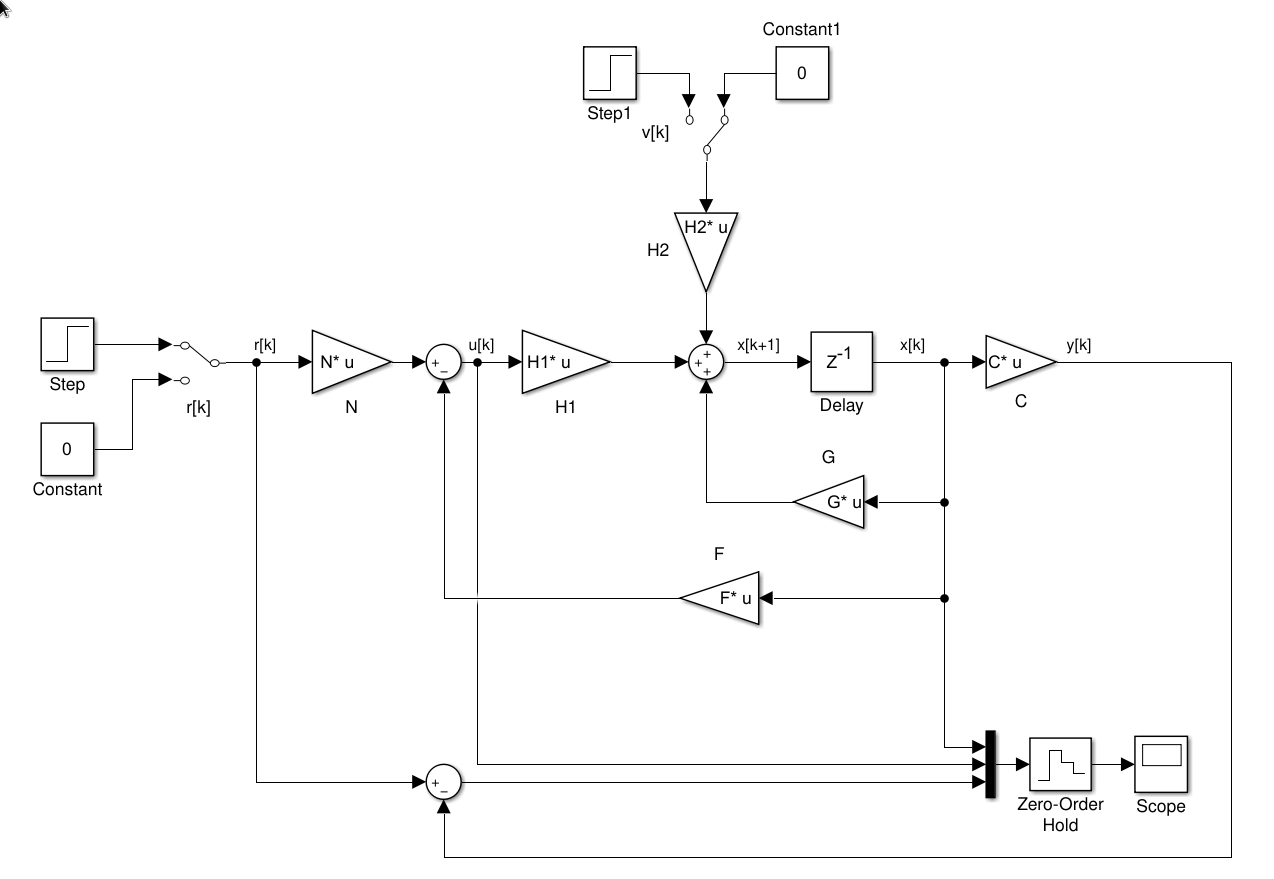
\includegraphics[width=.8\linewidth]{images/simulink_q1.png}
        \caption{Diagrama do sistema no Simulink.}\label{fig:simulink_q1}
    \end{figure}

    \begin{figure}[H]
        \centering
        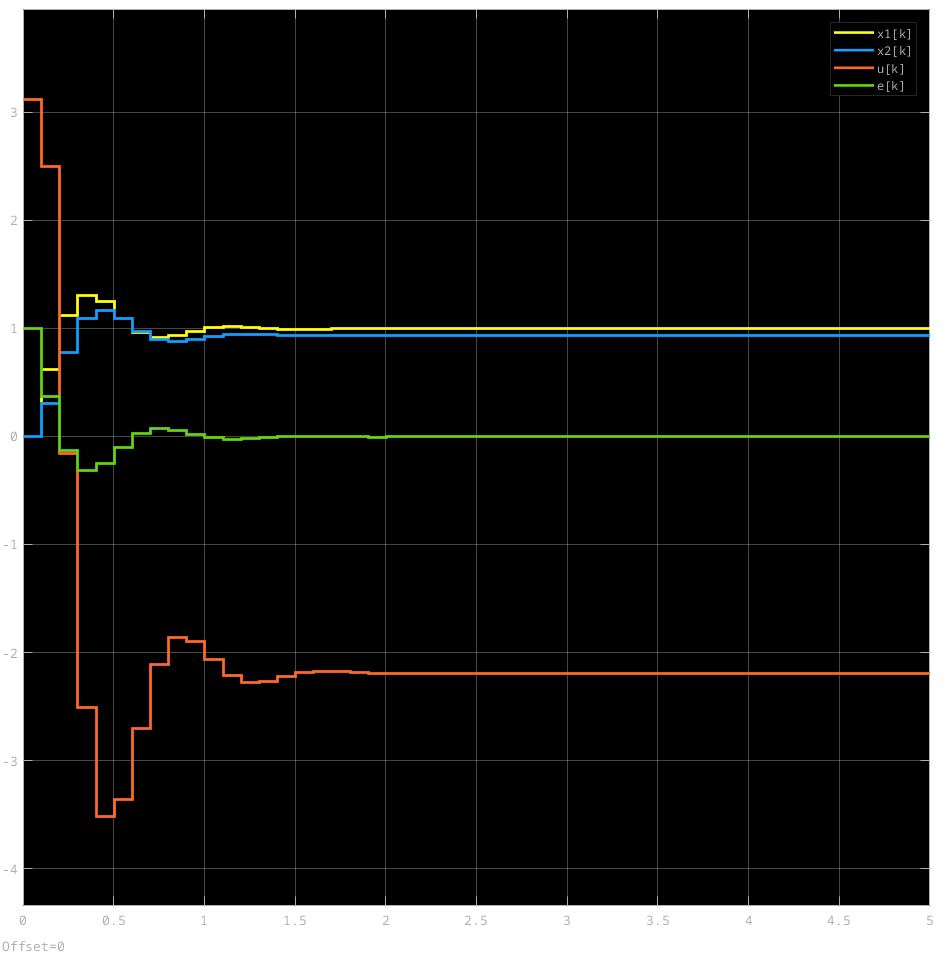
\includegraphics[width=.6\linewidth]{images/q1_r1_v0.png}
        \caption{Gráficos para $r[k]$ degrau unitário e $v[k]=0$.}\label{fig:q1_r1_v0}
    \end{figure}

    \begin{figure}[H]
        \centering
        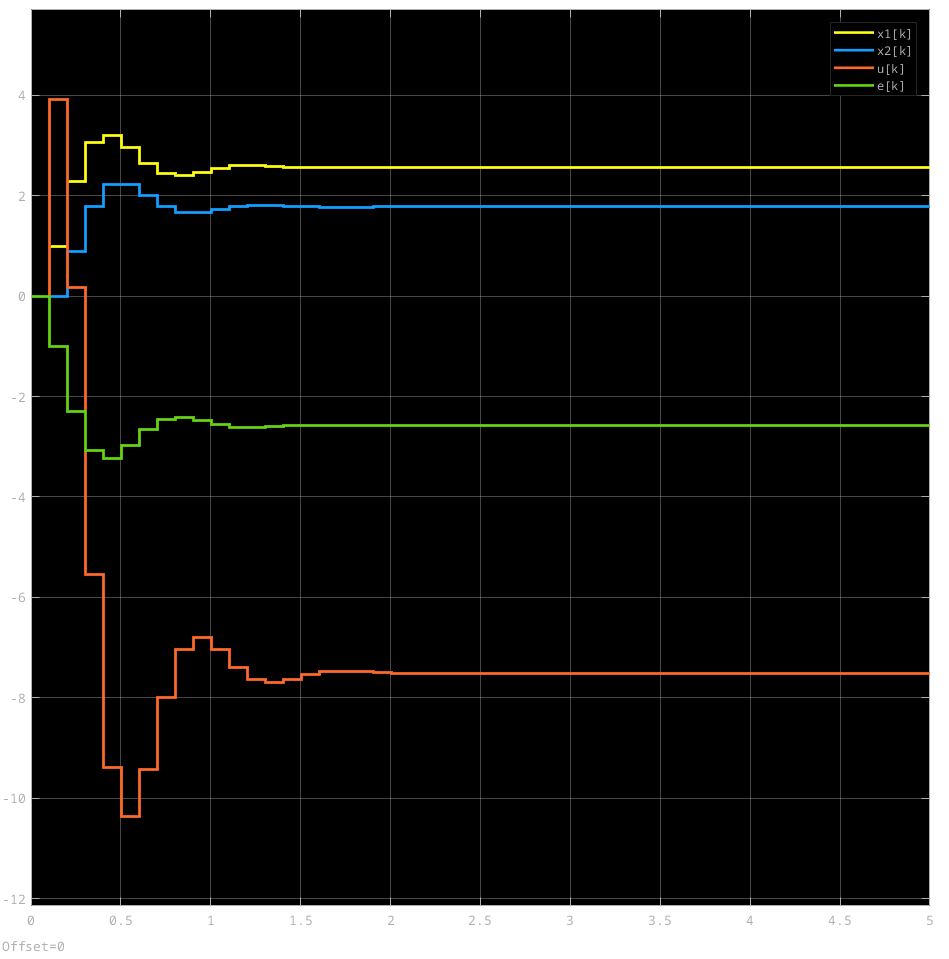
\includegraphics[width=.6\linewidth]{images/q1_r0_v1.png}
        \caption{Gráficos para $r[k]=0$ e $v[k]$ degrau unitário.}\label{fig:q1_r0_v1}
    \end{figure}


\clearpage
\section{\normalsize \normalfont{Determine uma realimentação de estados
$u[k] = f_ax_a[k] - Fx[k]$, onde $x_a[k+1] = x_a[k] +r[k] -y[k]$, de modo que
os polos de malha fechada fiquem em $z = 0.5 \pm j0.5$ e $z = 0$. Simule o
sistema para $r[k]$ degrau unitário e $v[k] = 0$, e para $r[k] = 0$ e $v[k]$
degrau unitário. Para cada simulação, apresente os gráficos de
$x_1[k]$, $x_2[k]$, $u[k]$ e $e[k] = r[k] - y[k]$:}}

    \begin{figure}[H]
        \centering
        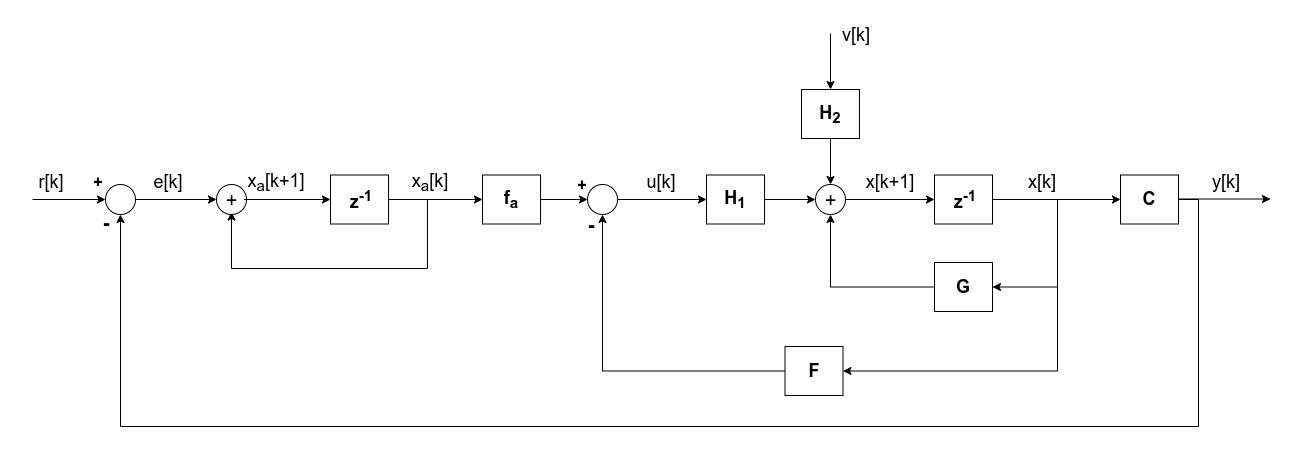
\includegraphics[width=1\linewidth]{images/diagram_q2.png}
        \caption{Diagrama do sistema.}\label{fig:diagram_q2}
    \end{figure}

    {Considerando condições iniciais nulas de $x[0]$,}
    \[ u[k] = f_ax_a[k] - Fx[k];\quad
        x_a[k+1] = x_a[k] + r[k] - y[k] = x_a[k] + e[k];\quad
        y[k] = Cx[k]
    \]
    {Fazendo a transformada $\mathcal{Z}$ de $x_a[k+1]$ considerando $x_a[0] = 0$,}
    \[ zX_a(z) - x_a[0] = X_a(z) +R(z) - Y(z) \implies X_a(z) = \frac{R(z)-Y(z)}{z-1} \]

    \[ x[k+1] = Gx[k] + H_1(f_ax_a[k] - Fx[k]) +H_2v[k] = (G-H_1F)x[k] + H_1f_ax_a[k] + H_2v[k] \]
    {Fazendo a transformada $\mathcal{Z}$ de $x[k+1]$ considerando $x[0] = 0$,}
    \[ zX(z) - x[0] = (G - H_1F)X(z) + H_1f_aX_a(z) + H_2V(z) \]
    \[ X(z) = (zI -G +H_1F)^{-1} (H_1f_aX_a(z) + H_2V(z)) \]
    \[ Y(z) = CX(z) = C(zI -G +H_1F)^{-1} (H_1f_aX_a(z) + H_2V(z))
        = \frac{C\adj(zI -G +H_1F)}{\det(zI -G +H_1F)}\left( \frac{H_1f_a(R(z) - Y(z))}{z-1} + H_2V(z) \right)
    \]
    \[ Y(z) = \frac{C\adj(zI -G +H_1F)H_1f_aR(z)}{\det(zI -G +H_1F)(z-1)}
            - \frac{C\adj(zI -G +H_1F)H_1f_aY(z)}{\det(zI -G +H_1F)(z-1)}
            + \frac{C\adj(zI -G +H_1F)H_2V(z)}{\det(zI -G +H_1F)}
    \]

    {Isolando $Y(z)$,}
    \[ Y(z) = \frac{C\adj(zI -G +H_1F)(H_1f_aR(z)+(z-1)H_2V(z))}
                   {\det(zI -G +H_1F)(z-1)+C\adj(zI -G +H_1F)H_1f_a}
    \]

    {Para $v[k] = 0$,}
    \[ \frac{Y(z)}{R(z)} = \frac{C\adj(zI -G +H_1F)H_1f_a}
            {\det(zI -G +H_1F)(z-1)+C\adj(zI -G +H_1F)H_1f_a}
    \]

    {Os polos de malha fechada desejados são $\Delta_f(z) =
    (z -0.5 +j0.5)(z-0.5 -j0.5)z = z^3 -z^2 +0.5z = 0$.}
    \[ \Delta_f(z) = \det(zI -G +H_1F)(z-1)+C\adj(zI -G +H_1F)H_1f_a \]

    {Pelo Matlab,}
    \begin{lstlisting}
syms f1 f2 fa
F = [f1 f2]
delta_f2 = vpa(collect(det(z*eye(2) -G + H1*F)*(z-1) + C * adjoint(z*eye(2) -G + H1*F)*H1*fa, z))
    \end{lstlisting}

    \[ \Delta_f(z) = z^3 -z^2 +0.5z = z^3 + (0.2f_1 + 0.1f_2 -2.2)z^2
        +(-0.24f_1 -0.05f_2 + 0.2f_a + 1.05)z + (0.04f_1 -0.05f_2 - 0.04f_a + 0.15) = 0
    \]
    \[
        \begin{cases}
            0.2f_1 + 0.1f_2 -2.2 = -1 \implies f_1 = 6-0.5f_2 & \implies f_1 = 4.1071\\
            -0.24f_1 -0.05f_2 + 0.2f_a + 1.05 = 0.5 \implies 0.07f_2+0.2f_a = 0.89 & \implies f_a = 3.125\\
            0.04f_1 -0.05f_2 - 0.04f_a + 0.15 = 0 \implies 0.056f_2 = 0.212 & \implies f_2 = 3.7857
        \end{cases}
    \]
    \[ u[k] = 3.125x_a[k] - [4.1071\quad 3.7857]
        \begin{bmatrix}
            x_1[k]\\
            x_2[k]
        \end{bmatrix}
    \]

    {Simulando o sistema da Figura~\ref{fig:simulink_q2} no Simulink, obtemos a
    resposta da Figura~\ref{fig:q2_r1_v0} para $r[k]$ degrau unitário e $v[k]=0$,
    e a resposta da Figura~\ref{fig:q2_r0_v1} para $r[k]=0$ e $v[k]$ degrau unitário.}

    \begin{figure}[H]
        \centering
        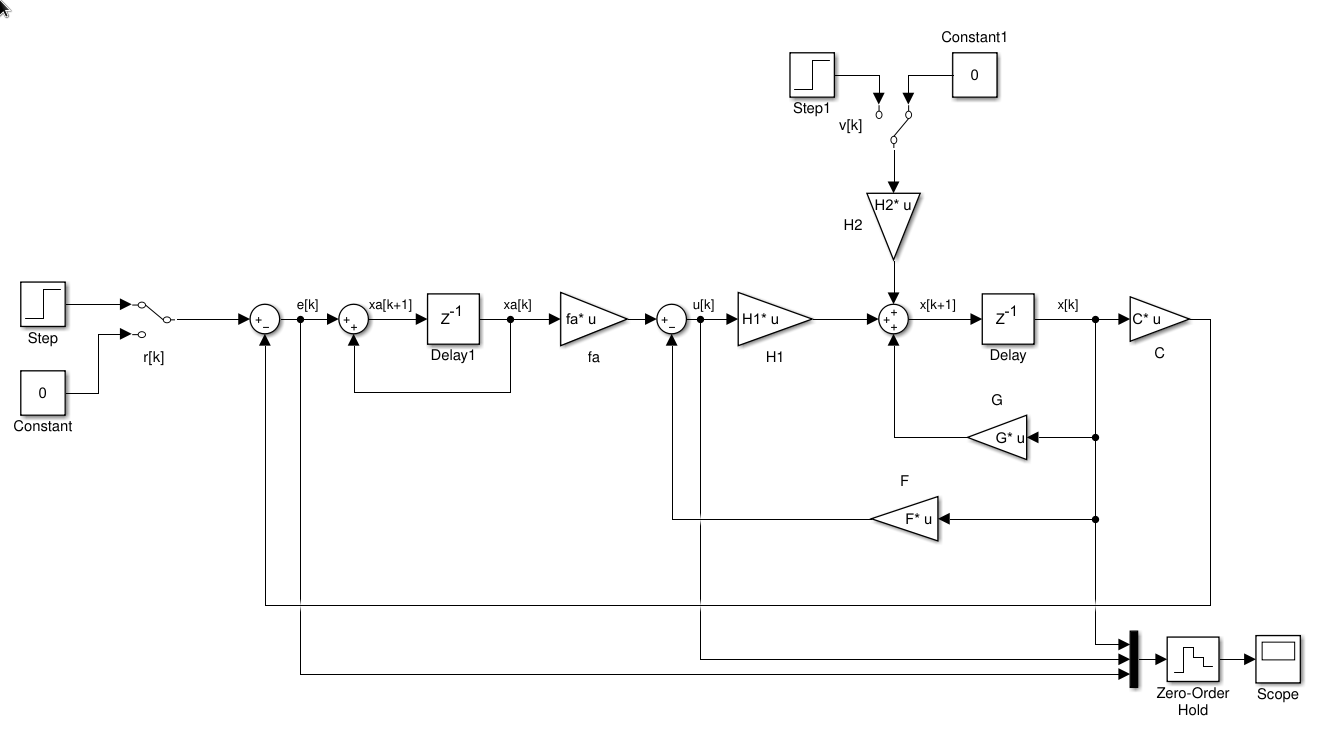
\includegraphics[width=1\linewidth]{images/simulink_q2.png}
        \caption{Diagrama do sistema no Simulink.}\label{fig:simulink_q2}
    \end{figure}

    \begin{figure}[H]
        \centering
        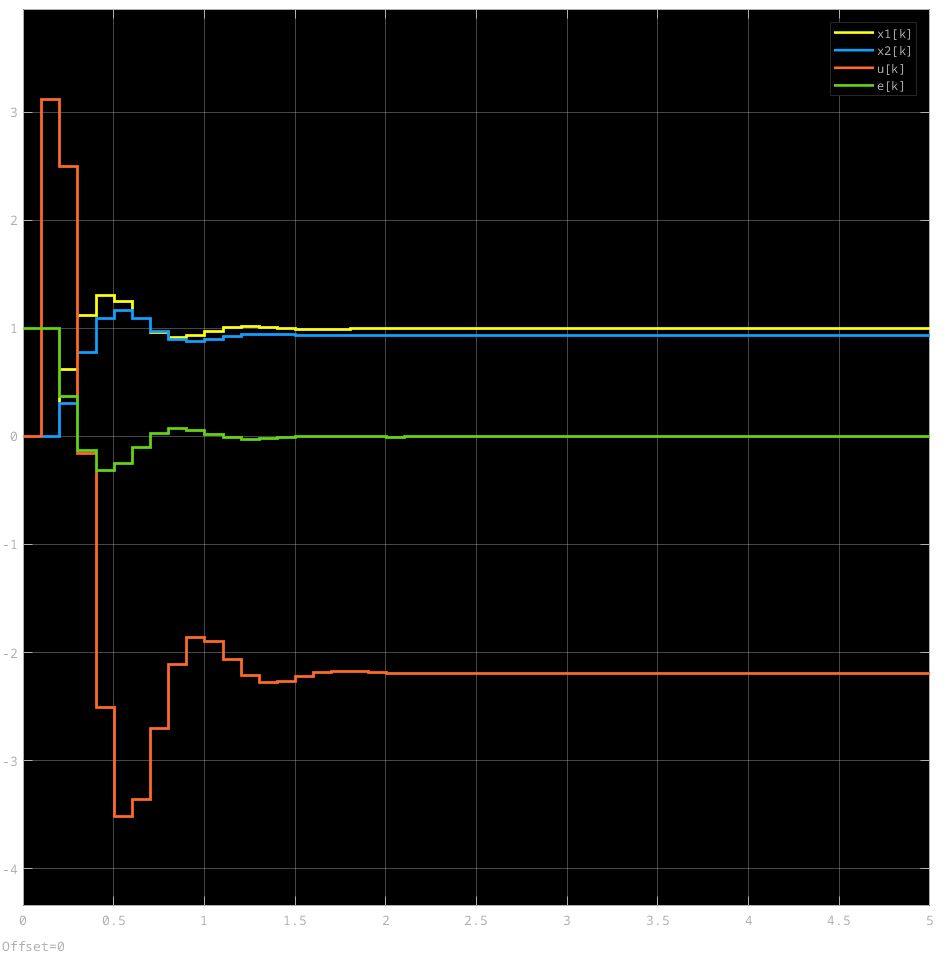
\includegraphics[width=.6\linewidth]{images/q2_r1_v0.png}
        \caption{Gráficos para $r[k]$ degrau unitário e $v[k]=0$.}\label{fig:q2_r1_v0}
    \end{figure}

    \begin{figure}[H]
        \centering
        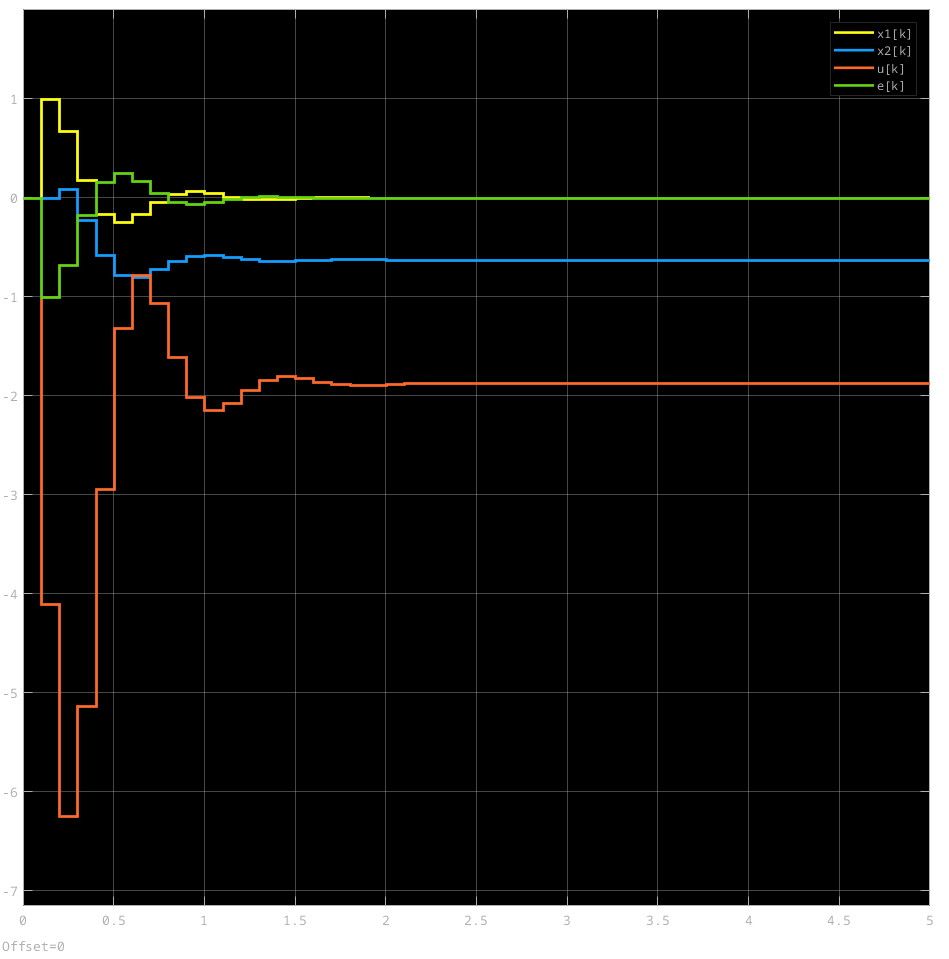
\includegraphics[width=.6\linewidth]{images/q2_r0_v1.png}
        \caption{Gráficos para $r[k]=0$ e $v[k]$ degrau unitário.}\label{fig:q2_r0_v1}
    \end{figure}


\clearpage
{Para o sistema com a segunda realimentação de estados e considerando que apenas
$y[k]$ é medido:}
\section{\normalsize \normalfont{Projete um observador de estados
$\tilde{x}[k+1] = G\tilde{x}[k] + H_1u[k] + L(y[k] - C\tilde{x}[k])$ com polos
em $z = 0.2 \pm j0.2$:}}

    \begin{figure}[H]
        \centering
        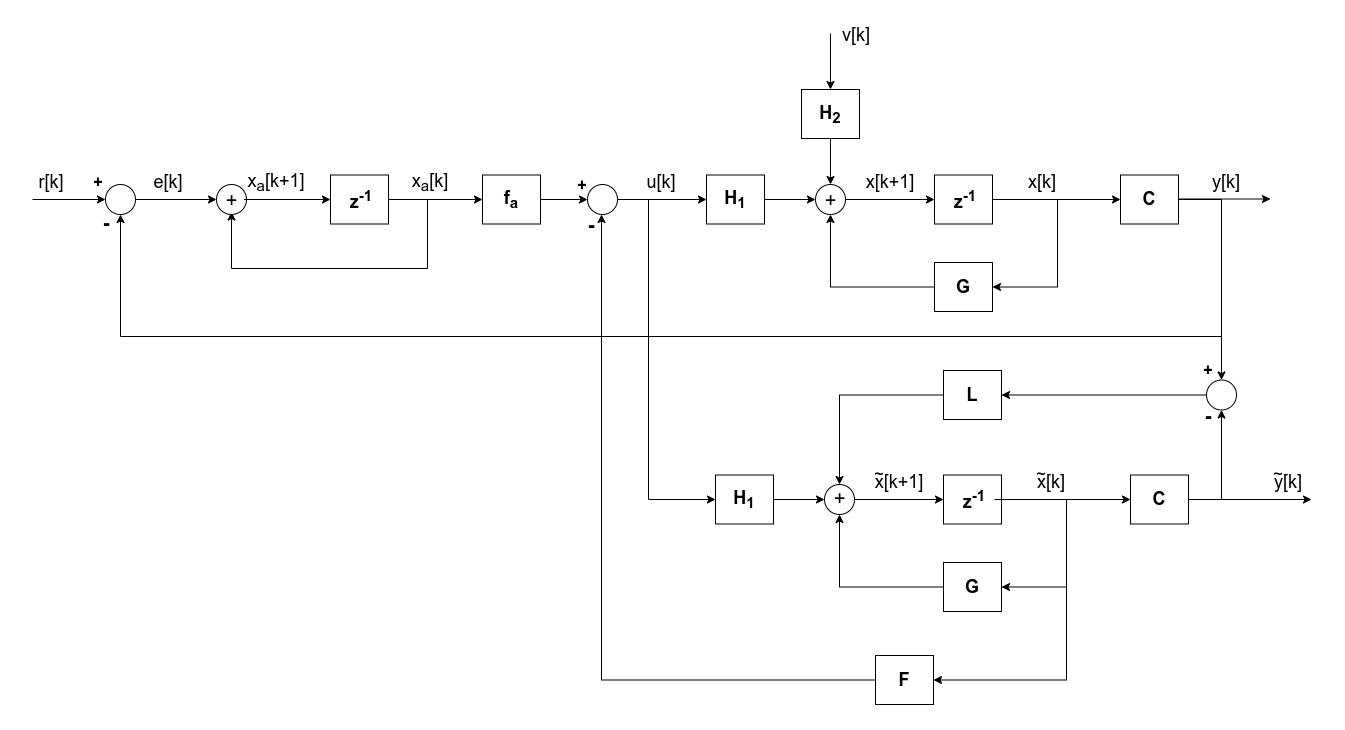
\includegraphics[width=1\linewidth]{images/diagram_q3.png}
        \caption{Diagrama do sistema.}\label{fig:diagram_q3}
    \end{figure}

    {Para que o sistema seja observável, $\det \mathscr{O} \ne 0$}
    \[ \mathscr{O} =
        \begin{bmatrix}
            C\\
            CG
        \end{bmatrix} =
        \begin{bmatrix}
            1 && 0\\
            0.5 && 1
        \end{bmatrix};\quad
        \det \mathscr{O} = 1
    \]
    {Assim, o par $(G, C)$ é observável.}

    {Os polos desejados do observador de estados são}
    \[ \Delta_o(z) = (z -0.2 +j0.2)(z-0.2 -j0.2) = z^2 -0.4z +0.08 = 0 \]

    \[ \tilde{y}[k] = C \tilde{x}[k] \]
    \[ \tilde{x}[k+1] = G\tilde{x}[k] + H_1u[k] + L(y[k] - C\tilde{x}[k]) =
        (G-LC)\tilde{x}[k] + H_1u[k]
    \]

    {Fazendo a transformada $\mathcal{Z}$,}
    \[ z\tilde{X}(z) - \tilde{x}[0] = (G-LC)\tilde{X}(z) + H_1U(z) \]
    \[ \tilde{X}(z) = (zI -G +LC)^{-1}H_1U(z) \]

    \[ \tilde{Y}(z) = C\tilde{X}(z) = C(zI -G +LC)^{-1}H_1U(z) \]
    \[ \frac{\tilde{Y}(z)}{U(z)} = C(zI -G +LC)^{-1}H_1
        = \frac{C \adj(zI -G +LC)H_1}{\det(zI -G +LC)}
    \]

    {Com $L = [l_1\quad l_2]^T$, usando o Matlab,}
    \begin{lstlisting}
syms l1 l2
L = [l1; l2]
delta_o = vpa(collect(det(z*eye(2) -G + L*C), z))
    \end{lstlisting}

    \[ \Delta_o(z) = \det(zI -G +LC) = z^2 + (l_1 -1.2)z +(-0.7l_1 + l_2 -0.15) =
        z^2 -0.4z +0.08 = 0
    \]
    \[
        \begin{cases}
            l_1 - 1.2 = -0.4 & \implies l_1 = 0.8\\
            -0.7l_1 + l_2 -0.15 = 0.08 & \implies l_2 = 0.79
        \end{cases}
    \]
    \[ L = \begin{bmatrix}
            0.8\\
            0.79
        \end{bmatrix}
    \]


\section{\normalsize \normalfont{Simule o sistema em malha fechada com o
observador de estados, $r[k] = 0$, $v[k] = 0$, $x[0] = [1\quad -1]^T$ e
$\tilde{x}[0] = [0\quad 0]^T$. Apresente gráficos de $x_1[k]$, $\tilde{x}_1[k]$,
$x_2[k]$, $\tilde{x}_2[k]$, $u[k]$ e $e[k]$:}}

    {Simulando o sistema da Figura~\ref{fig:simulink_q4} no Simulink, obtemos a
    resposta da Figura~\ref{fig:q4_r0_v0} para $r[k]=v[k]=0$,
    $\tilde{x}[0] = [0 0]^T$ e $x[0] = [1\quad -1]^T$.}

    \begin{figure}[H]
        \centering
        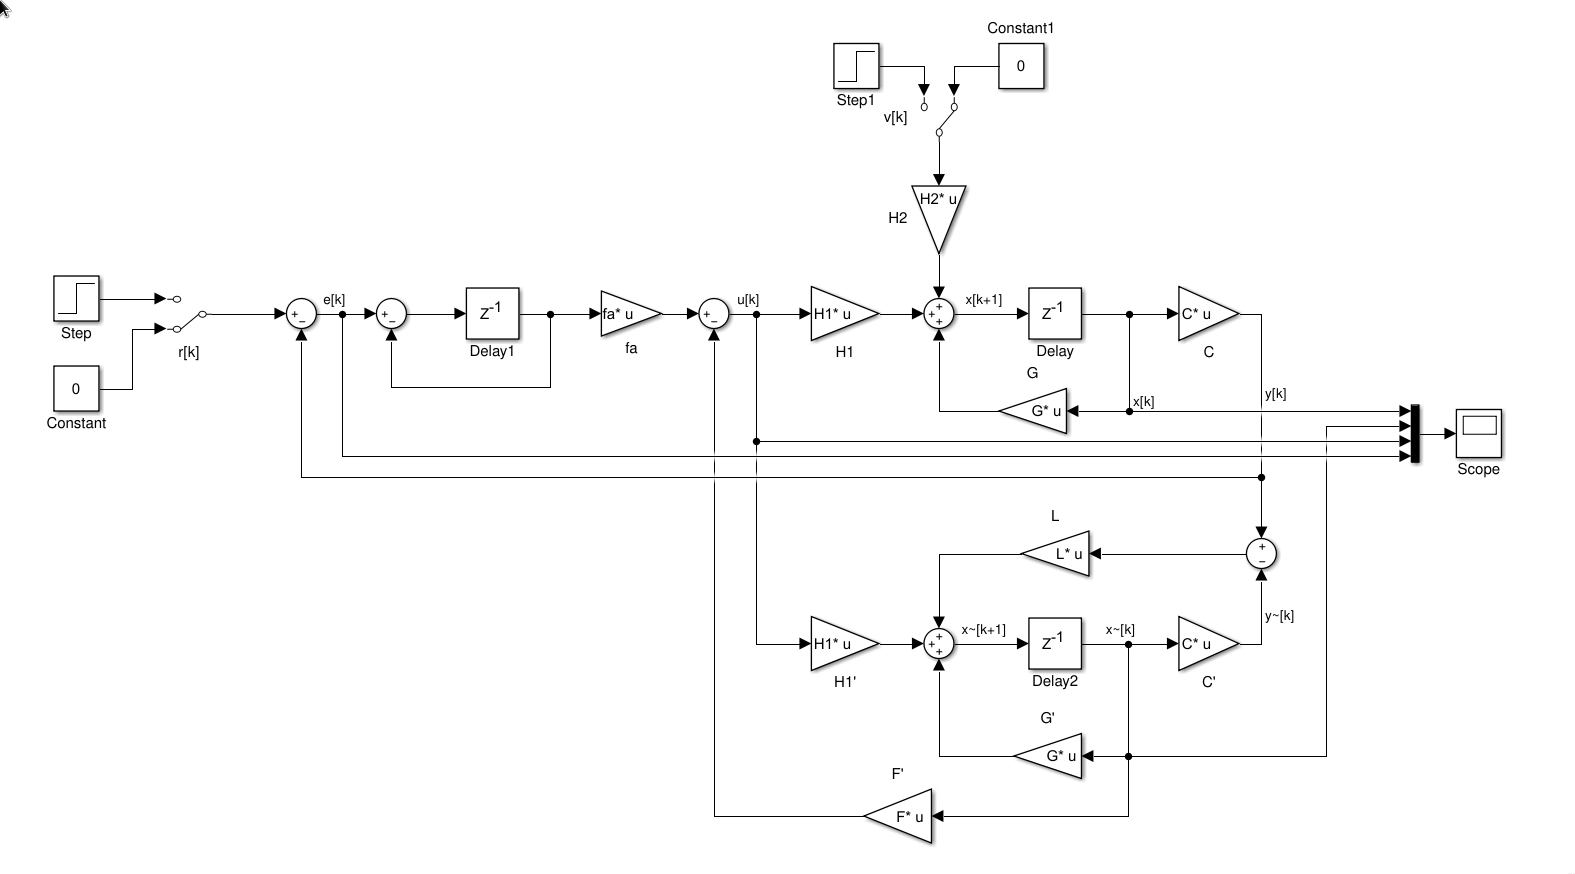
\includegraphics[width=1\linewidth]{images/simulink_q4.png}
        \caption{Diagrama do sistema no Simulink.}\label{fig:simulink_q4}
    \end{figure}

    \begin{figure}[H]
        \centering
        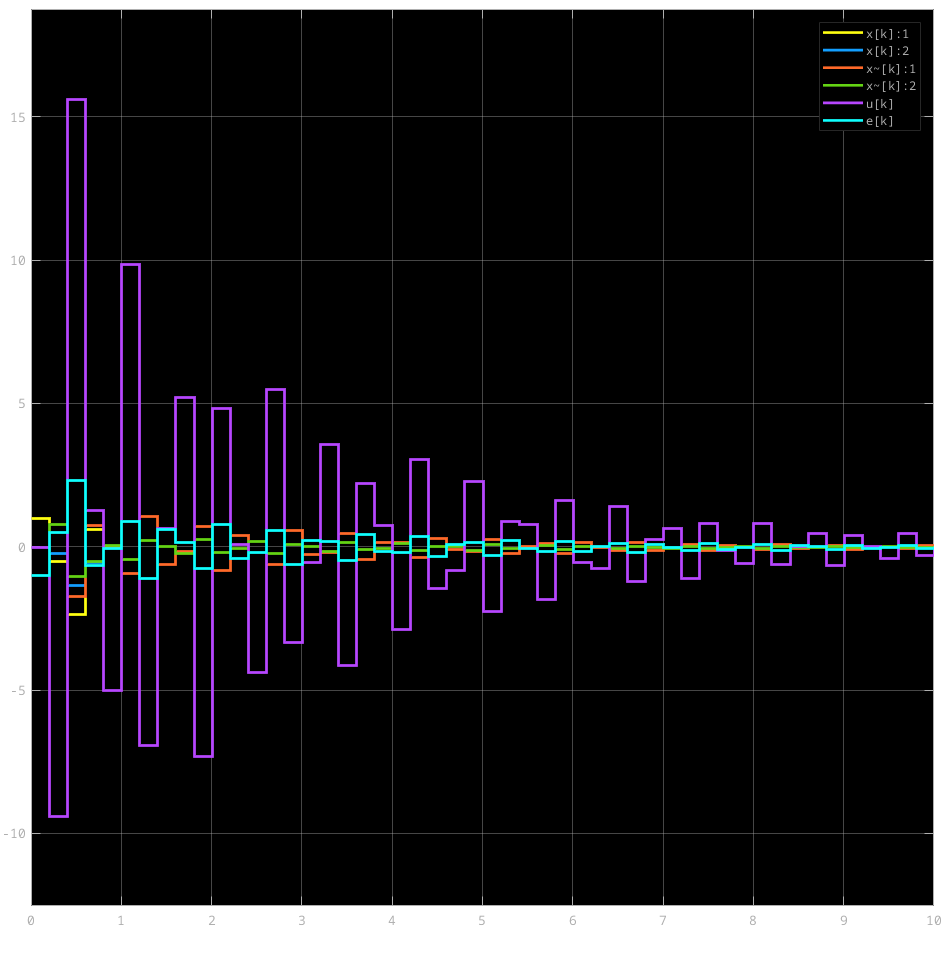
\includegraphics[width=.6\linewidth]{images/q4_r0_v0.png}
        \caption{Gráficos para $r[k]=v[k]=0$ com $x[0] = [1\quad -1]^T$ e $\tilde{x}[0] = [0\quad 0]^T$.}\label{fig:q4_r0_v0}
    \end{figure}


\section{\normalsize \normalfont{Simule o sistema em malha fechada com o
observador de estados, $r[k] = 0$, $v[k]$ degrau unitário,
$x[0] = \tilde{x}[0] = [0\quad 0]^T$. Apresente gráficos de
$x_1[k]$, $\tilde{x}_1[k]$, $x_2[k]$, $\tilde{x}_2[k]$, $u[k]$ e $e[k]$:}}


    {Simulando o sistema da Figura~\ref{fig:simulink_q5} no Simulink, obtemos a
    resposta da Figura~\ref{fig:q5_r0_v1} para $r[k]=0$ e $v[k]$ degrau unitário.}

    \begin{figure}[H]
        \centering
        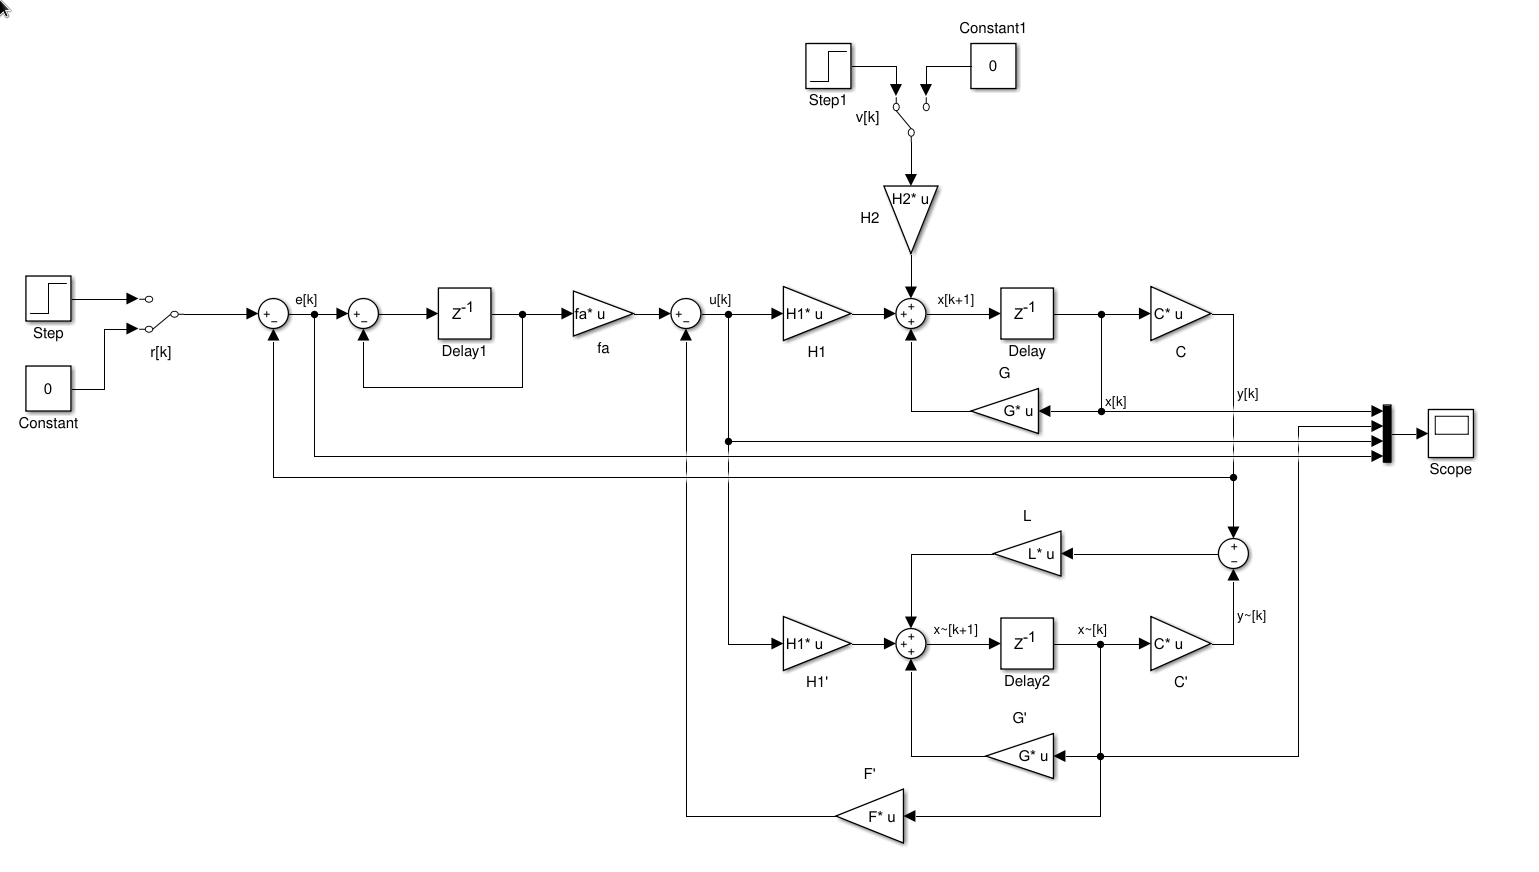
\includegraphics[width=.8\linewidth]{images/simulink_q5.png}
        \caption{Diagrama do sistema no Simulink.}\label{fig:simulink_q5}
    \end{figure}

    \begin{figure}[H]
        \centering
        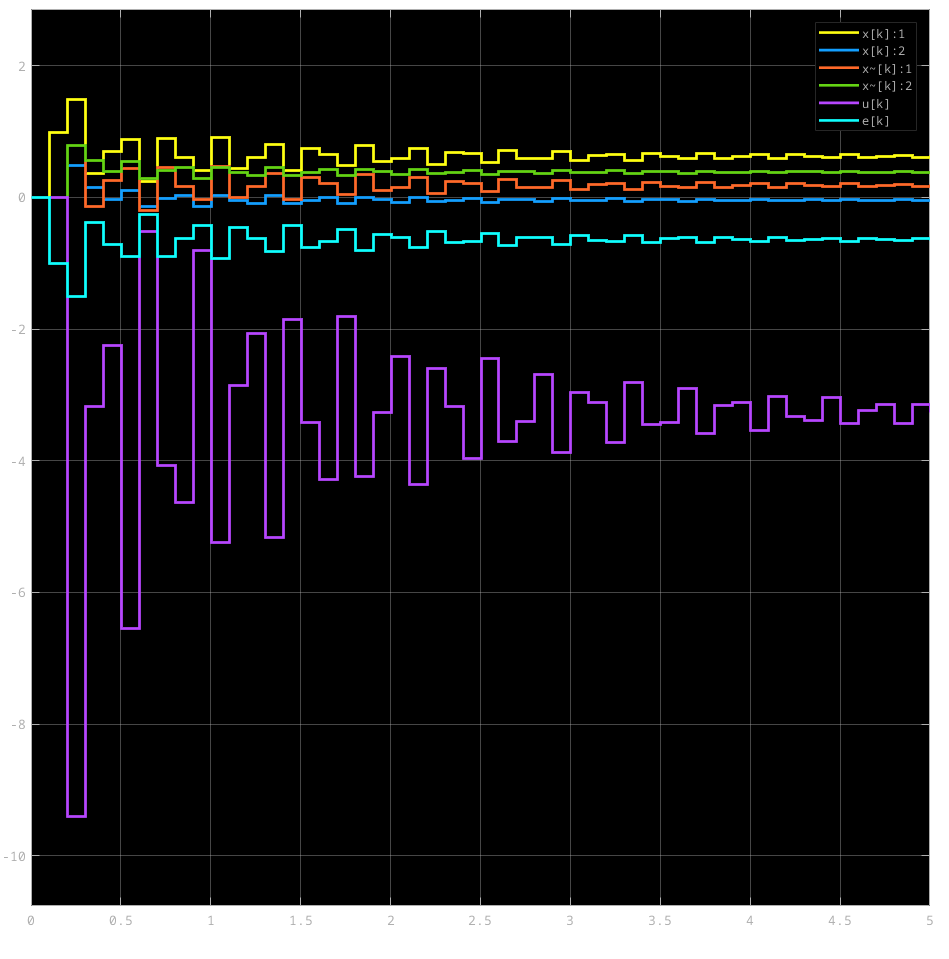
\includegraphics[width=.6\linewidth]{images/q5_r0_v1.png}
        \caption{Gráficos para $r[k] = 0$ e $v[k]$ degrau unitário com $x[0] = \tilde{x}[0] = [0\quad 0]^T$.}\label{fig:q5_r0_v1}
    \end{figure}


\end{document}

